\section{Human Resource Allocation}
\label{DDHR}
The first part of the project will involve a team of five specialists designing the five critical subsystems and one person designing the orbits of the swarm. The other four members will concentrate on the development of the software that will be used to assist the trade-off and verify the design. At later stages, some of the the software engineering personnel will be heavily involved in designing proper algorithms for the processing of mission data, while others will be brought in to assist with detail design. 

A schematic representation of the resource allocation can be found in figure \ref{fig:DDBBHR} on page \pageref{fig:DDBBHR}.

\begin{figure}[ht!]
\begin{center}
\includegraphics[width=0.9\textwidth]{chapters/img/HR.png}
\label{fig:DDBBHR}
\caption{Human resource allocation chart}
\end{center}
\end{figure}

%%%%%%%%%%%%%%%%%%%%%%%%%%%%%%%%%%%%%%%%%%%%%%%%%%%%%%%%%%%%%%%%%%%%%%%%%%%%%%%%%%%%

\section{Mass Budget Breakdown}
\label{sect_mass_budget}
A satellite is built up from a number of subsystems, which all have a mass. Figure \ref{massbreakdown} on page \pageref{massbreakdown} shows the different subsystems and some examples of components that contribute to the mass of the subsystem. In table \ref{rotsubsystemmass} rules of thumb for finding the mass of the different subsystems are given in terms of the satellite's dry mass. It has to be noted that the rules mainly count for conventional satellites. When using micro- or even nano-satellites there might be another distribution of mass, since some systems like computers can be miniaturized, while other systems like antennas can not. 

\begin{figure} [ht]
\centering
\includegraphics[width=0.7\textwidth]{chapters/img/mass_breakdown.png}
\label{massbreakdown}
\caption{Mass Budget Breakdown Structure}
\end{figure}

\begin{table} [h]
\centering
\begin{tabular}{p{12cm} | l | l}
\textbf{SUBSYSTEM} & \textbf{$\%$ OF M\textsubscript{dry}} & \textbf{SOURCE} \\ \hline \hline
Propulsion & 2.5-7 \% & \cite{Space2b} \\ 
\ac{ADCS} (incl. \ac{GNC}) & 3-9 \% & \cite{Space2b} \\ 
\ac{CDH} and \ac{TTC} & 2.5-7 \% & \cite{Space2b} \\ 
Thermal & 3 \% & \cite{larson} \\ 
Power & 20-40 \% & \cite{Space2b} \\ 
Structure \& Mechanics & 18-25 \% & \cite{Space2b} \\ 
Payload & 15-50 \% & \cite{larson} 
\end{tabular} 
\caption{Mass budget breakdown estimation of subsystem mass, in terms of dry mass}
\label{rotsubsystemmass}
\end{table}

%%%%%%%%%%%%%%%%%%%%%%%%%%%%%%%%%%%%%%%%%%%%%%%%%%%%%%%%%%%%%%%%%%%%%%%%%%%%%%%%%%%%

\section{Power Budget Breakdown}
\label{blBudgetPower}

At this preliminary stage, the power budget breakdown is an estimation based on previous missions and on general data taken from \cite{larson}.

The biggest power requirements come from the mission payload and the power system. The payload needs power to be able to operate the emitter
and the receiver for the whole mission lifetime. About 30$\%$ of the total power will be used to operate the transmitter and 10$\%$ for the receiver. The power distribution and control will take up about 30$\%$ of all the power. Of this 25$\%$ will be needed for the regulators and converters and 5$\%$ will be lost due to wiring losses during the distribution of the power. Furthermore, the \ac{ADCS} system will need approximately 15$\%$ of the total power to be able to operate. The amount of power that will go to its subsystems (sensors, controllers and processors) is an estimate based on previous missions (i.e. FireSat \cite{larson}).

The last subsystem that needs power is Communications. This system is divided further in to the actual communications and the command and data handling subsystem. Each receive about 5$\%$ of the total power. The power distribution for the transmitter and receiver was taken from values of typical X-Band, S-Band and Ku-Band communication subsystems.
For the power distribution of the command and the telemetry unit, average nominal values were used \cite{larson}.

The power breakdown structure and the corresponding power allocation for each system can be seen in figure \ref{fig:powerbudget} on page \pageref{fig:powerbudget}. A tabulated representation of the breakdown estimations can be found in table \ref{epsbudgettable}.

\begin{table} [h]
\centering
\begin{tabular}{p{12cm} | l }
\textbf{SUBSYSTEM} & \textbf{$\%$ OF TOTAL} \\ \hline \hline
\ac{ADCS} & 15  \\
\hspace{1.0cm} Sensor & 3 \\
\hspace{1.0cm} Controllers & 8 \\
\hspace{1.0cm} Processors & 4 \\ 
\ac{CDH} and \ac{TTC} & 10  \\
\hspace{1.0cm} Communications & 5 \\
\hspace{1.0cm} \hspace{1.0cm} Receiver & 1 \\
\hspace{1.0cm} \hspace{1.0cm} Transmitter & 4 \\
\hspace{1.0cm} Data Handling & 5 \\ 
\hspace{1.0cm} \hspace{1.0cm} Command Unit & 1 \\
\hspace{1.0cm} \hspace{1.0cm} Telemetry & 4 \\
Power & 30 \\
\hspace{1.0cm} Regulator/Converters & 25 \\
\hspace{1.0cm} Wiring & 5 \\
Payload & 40\\
\hspace{1.0cm} Emitter & 30 \\
\hspace{1.0cm} Emitter & 10 \\
\end{tabular} 
\caption{Power budget breakdown estimation}
\label{epsbudgettable}
\end{table}

\begin{figure}
\centering
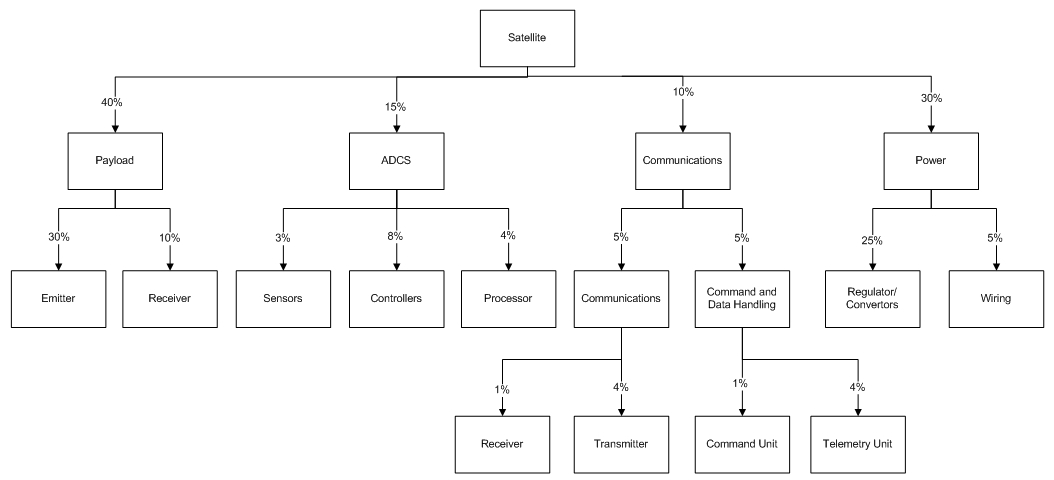
\includegraphics[width=0.9\textwidth, angle=90]{chapters/img/Power_budget_breakdown.jpg}
\caption{Power Budget Breakdown Structure}
\label{fig:powerbudget}
\end{figure}

%%%%%%%%%%%%%%%%%%%%%%%%%%%%%%%%%%%%%%%%%%%%%%%%%%%%%%%%%%%%%%%%%%%%%%%%%%%%%%%%%%%%%%%%%%%%

\section{Cost Budget Breakdown}
\label{blBudgetCost}
For a preliminary estimation of cost breakdown it is necessary to realize the different stages of the life-cycle costs. These are the costs of the entire space mission from the first stages of planning until end of life.
%
%\begin{wrapfigure}{L}{1\textwidth}[H]
%	\begin{center}
%  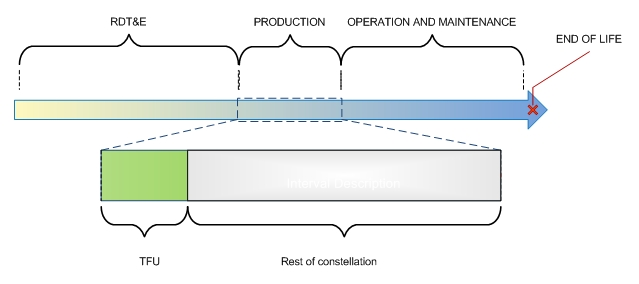
\includegraphics[width=1\textwidth]{chapters/img/lifetime.jpg}
%  \end{center}
%  \caption{Life-Cycle}
%  \label{fig:lifecycle}
%\end{wrapfigure}


Figure \ref{fig:lifecycle} on page \pageref{fig:lifecycle} shows a typical life-cycle for a space mission. The \ac{RDTE} stage includes the planning, development and testing of all prototypes and qualification units, but does not include the technology development for different subsystems. In the case of the laser swarm this is largely dependent on the single emitter and one receiver unit. This stage is also mostly consistent of non-recurring costs. The production stage consists of actual manufacture of the physical satellites. The cost estimation in this stage is based on the \ac{TFU}. This is done because it is assumed that the first unit (in the case of the Laser Swarm, that would be the emitter and one receiver) would be the most expensive to produce. The rest of the swarm constellation satellite costs are calculated by taking a theoretical learning curve \cite{larson}. 

\begin{figure}[!h]
\begin{center}

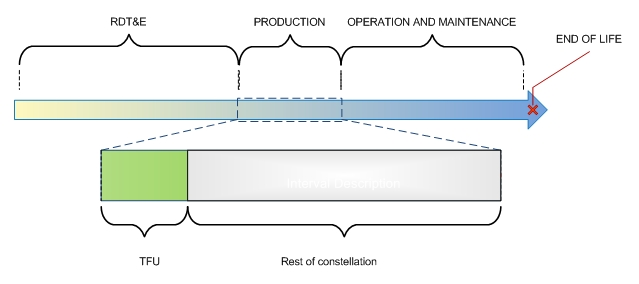
\includegraphics[width=0.7\textwidth]{chapters/img/lifetime.jpg}
\caption{Satellite Life-Cycle}
\label{fig:lifecycle}
\end{center}
\end{figure}

The final stage - \ac{OM} is self explanatory. This phase can be very expensive for large constellations. The ground segment is the prevailing factor.

The cost breakdown can be found in figure \ref{fig:costbreak} on page \pageref{fig:costbreak}. In this diagram, the cost is broken down into segments. This way it is easier to follow cost distribution down to all subsystems.

Because of the nature of the system that is being designed - as a collection of satellites - it is very hard to make an accurate prediction of costs before critical decisions have been made. Most subsystem costs are mass driven, so design options create a large margin of error in early estimates. Furthermore, due to the high cost of actual production of individual satellites, a swarm is hard to predict without a rough idea of the number of space platforms. It is important to note that cost is also dependent on so called heritage factors. These factors allow for reduction of costs based on already existing designs. However, if some kind of new technology is used in a subsystem then this reduction cannot be used.

Table \ref{tab:CostBreakdown} on page \pageref{tab:CostBreakdown} contains percentage estimations of all aspects covered in figure \ref{fig:costbreak}.


\begin{table*}[htbp]
	\centering

% Table generated by Excel2LaTeX from sheet 'Sheet1'
\begin{tabular}{p{10cm} | c | c }

   \textbf{SEGMENT} & \textbf{$\%$ OF PARENT} & \textbf{$\%$ OF TOTAL} \\ \hline \hline

\textsl{Space Segment} &          &       30   \\ \hline

      \hspace{1.0cm}RDTE &         30 &   9       \\ \hline

   \hspace{2.0cm}Payload &         26 &     2.3     \\

       \hspace{2.0cm}Bus &         52 &     4.7    \\ \hline

 \hspace{2.5cm}Structure &         24&      1.1    \\

  \hspace{2.5cm}Thermal &         2 &       0.1   \\

      \hspace{2.5cm}EPS &         22 &      1    \\

\hspace{2.5cm}Communications &         38 &      1.8    \\

      \hspace{2.5cm}ADCS &         14 &     0.7     \\ \hline

       \hspace{2.0cm}IAT &         0 &         0 \\

 \hspace{2.0cm}Program Level &         22 &       2   \\ \hline
 \hspace{2.5cm}Program Management &         20 &      0.4    \\
 \hspace{2.5cm}Systems Engineering &         40 &     0.8     \\
 \hspace{2.5cm}Product Assurance &         20 &       0.4   \\
 \hspace{2.5cm}System Evaluation &         20 &       0.4   \\ \hline

        \hspace{2.0cm}GSE &         4 &      0.4    \\

      \hspace{2.0cm}LOOS &         0 &         0 \\ \hline

  \hspace{1.0cm}Software &         25 &         7.5 \\

\hspace{1.0cm}Production &         45 &         13.5 \\ \hline

       \hspace{2.0cm}TFU &         10-30 &       1.4-4.8   \\ \hline

   \hspace{2.5cm}Payload &         20 &       0.3-0.8   \\

       \hspace{2.5cm}Bus &         45 &        0.6-1.8  \\ \hline

 \hspace{3.0cm}Structures &         24 &       0.1-0.4   \\

   \hspace{3.0cm}Thermal &         5 &         0.04-0.12 \\

       \hspace{3.0cm}EPS &         20 &        0.1-0.4  \\

\hspace{3.0cm}Communications &         18 &      0.1-0.3    \\

      \hspace{3.0cm}ADCS &         28 &         0.2-0.5 \\ \hline

       \hspace{2.5cm}IAT &         14&         0.2-0.6 \\

\hspace{2.5cm}Program Level &         13 &         0.2-0.5 \\ \hline
 \hspace{3.0cm}Program Management &         30 &       0.05-0.16   \\
 \hspace{3.0cm}Systems Engineering &         20 &        0.04-0.11  \\
 \hspace{3.0cm}Product Assurance &         30 &       0.05-0.16   \\
 \hspace{3.0cm}System Evaluation &         20 &       0.04-0.11   \\ \hline

       \hspace{2.5cm}GSE &         0 &          0\\

      \hspace{2.5cm}LOOS &         5 &         0.07-0.2 \\ \hline

     \hspace{2.0cm}Swarm &         70-90 &         9.5-12 \\ \hline

\textit{Launch Segment} &         &         5-10 \\ \hline

  \hspace{1.0cm}Launcher &         100 &        5-10  \\ \hline

\textit{Ground Segment} &          &     20     \\ \hline

\hspace{1.0cm}First Ground Station &         25 &      5    \\

\hspace{1.0cm}Consecutive Ground Stations &         55 &     11     \\

\hspace{1.0cm}Software &         20 &     4     \\ \hline

\textit{Operations and Maintenance} &          &        45  \\ \hline

\hspace{1.0cm}Operations and support of ground stations &         100 &   45       \\
	
\end{tabular} 
\caption{Cost budget breakdown estimations}
	\label{tab:CostBreakdown} 
\end{table*}

\begin{figure}[ht!]
\begin{center}

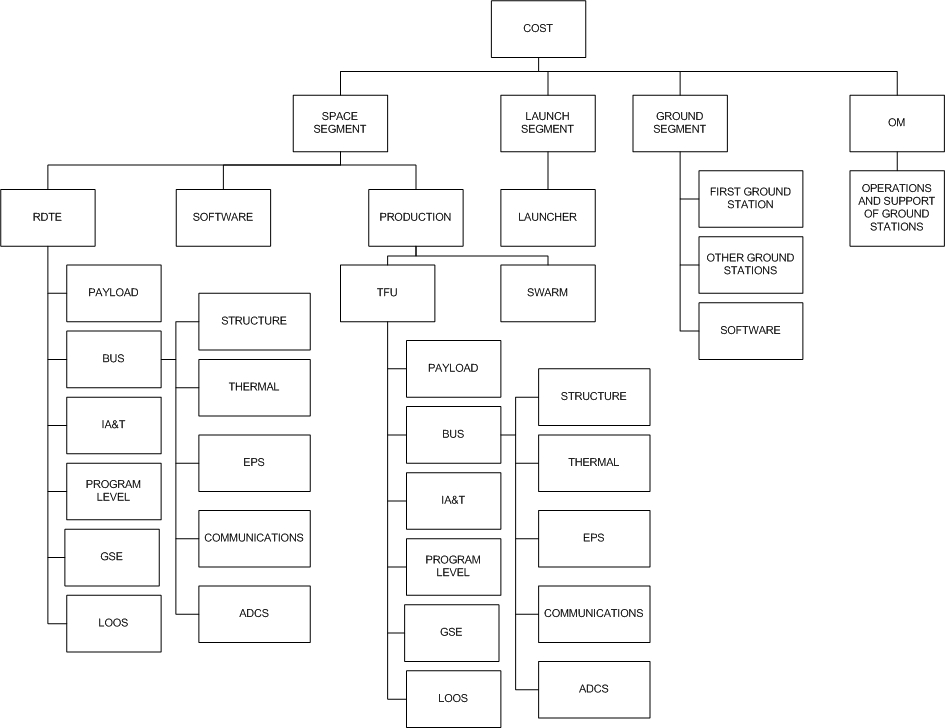
\includegraphics[height=0.8\textwidth,angle=90]{chapters/img/costbreakdown.jpg}
\caption{Cost Budget Breakdown Structure}
\label{fig:costbreak}
\end{center}
\end{figure}


